%-----------------------------------------------------------------------------%
% \addChapter{DAFTAR LAMPIRAN}
% \chapter*{Daftar Lampiran}
% %-----------------------------------------------------------------------------%
\newpage
% \appendix
% \appendices{Lampiran 1. Form Bimbingan} 

\appendices{Hasil Persentase Turnitin} 
\begin{center}
    \frame{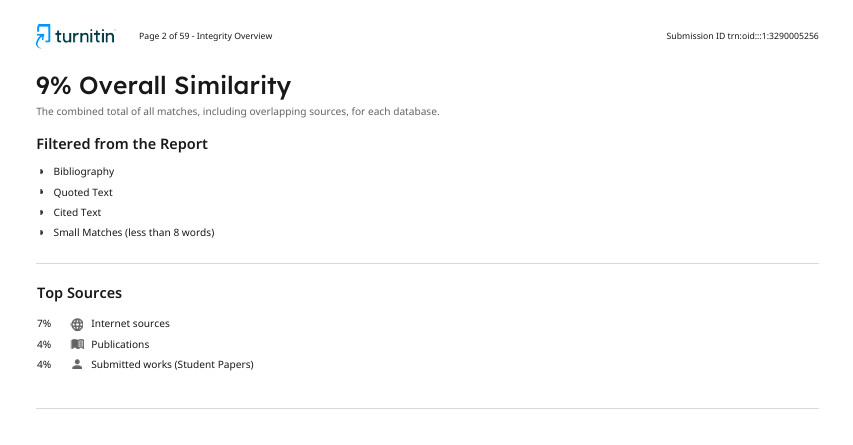
\includegraphics[width=\textwidth,page=1]{assets/pics/hasil_turnitin.png}}
\end{center}

\newpage

\appendices{Formulir Bimbingan} 
% \renewcommand{\thechapter}{Lampiran \alph{chapter}}
% \renewcommand{\thesection}{Lampiran \arabic{section}}

% \section*{Form Bimbingan}
% \addtocontents{apc}{\let\protect\l@chapter\protect\l@section}
% \addtocontents{apc}{section}
\begin{center}
    \frame{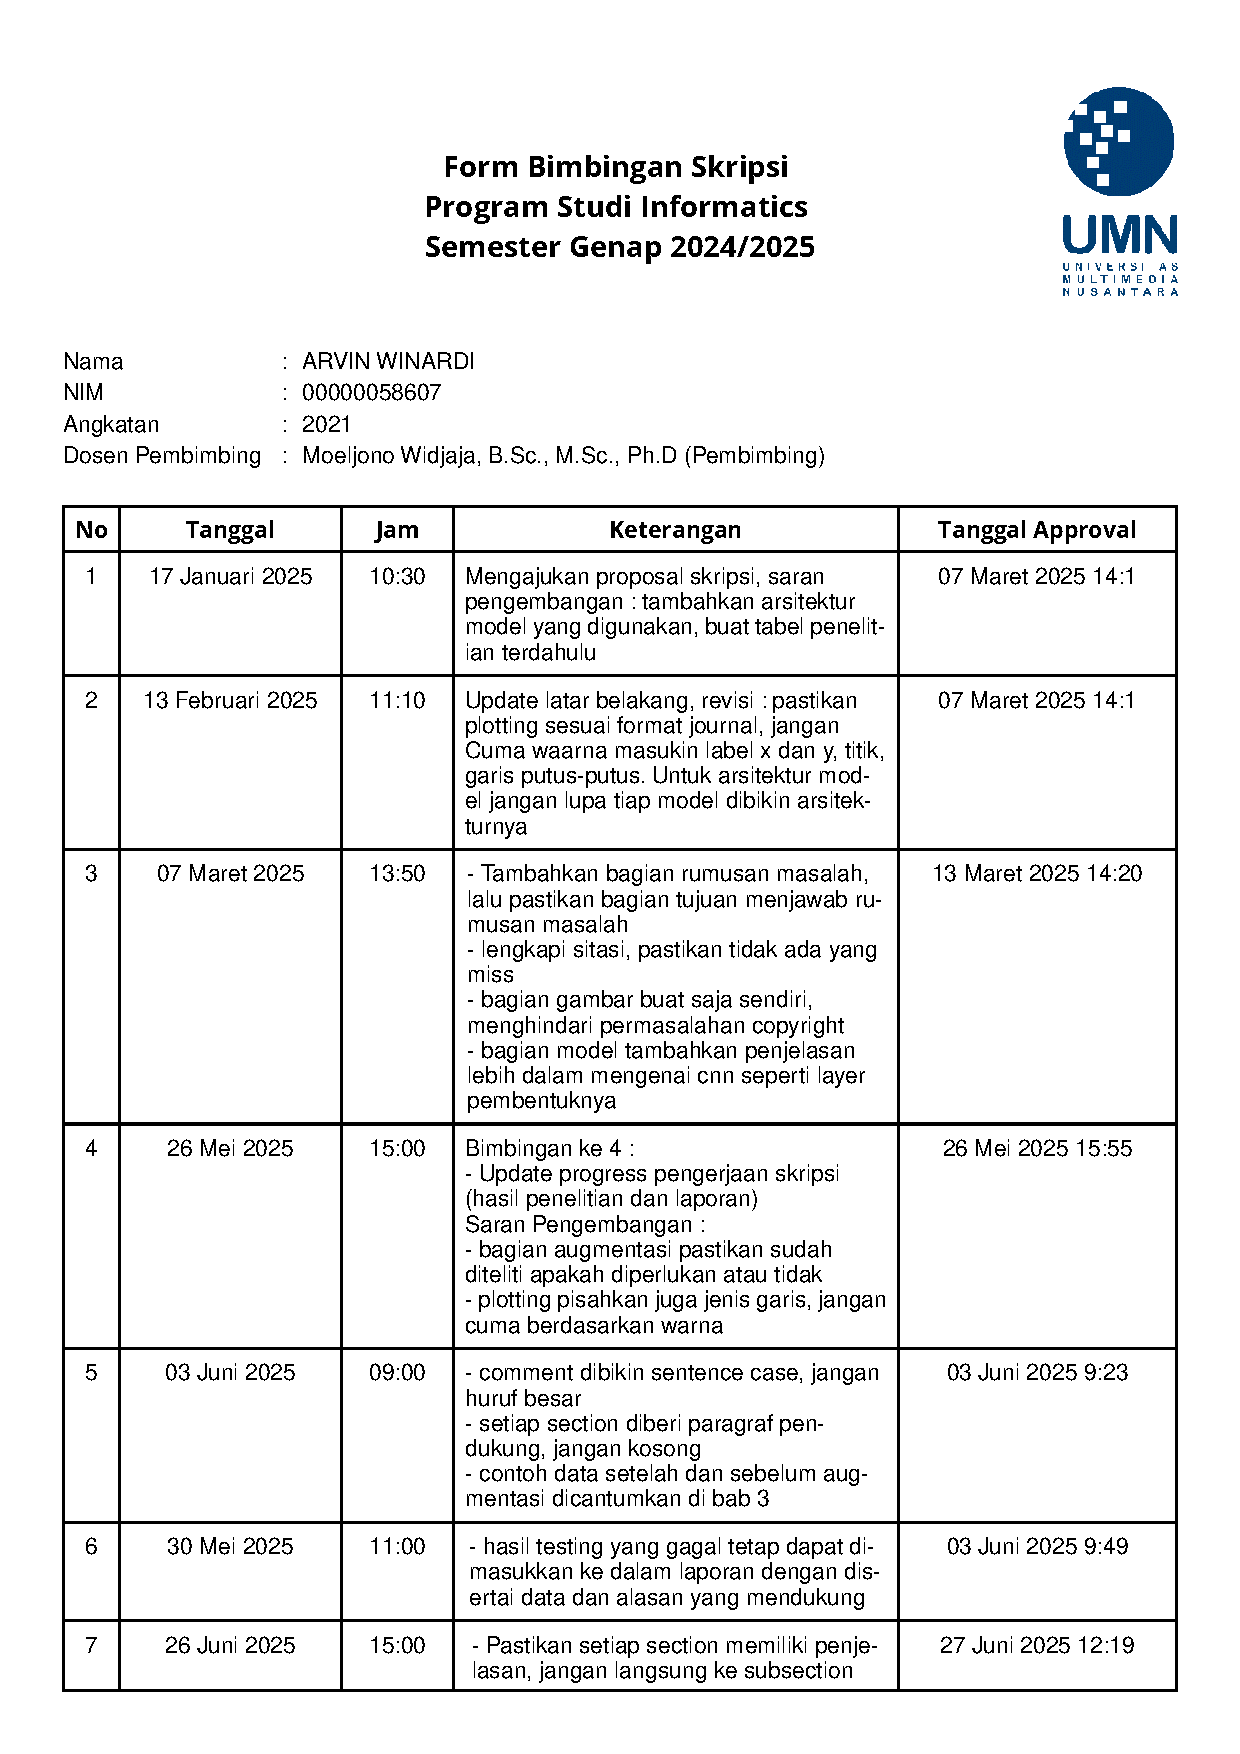
\includegraphics[width=\textwidth,page=1]{assets/pdf/Counseling Form .pdf}}
\end{center}
\clearpage

\newpage

\appendices{Perbandingan Metode Deteksi \textit{Deepfake}}

Tabel berikut menunjukkan perbandingan metode deteksi \textit{deepfake} terkini dengan berbagai arsitektur dan \textit{dataset} yang digunakan dalam literatur ilmiah.

\begin{table*}[h]
\centering
\caption{Perbandingan metode deteksi \textit{deepfake} dari berbagai penelitian}
\label{tab:deepfake_detection_appendix}
\resizebox{\textwidth}{!}{%
\begin{tabular}{lccccc}
\toprule
\textbf{Metode} & \textbf{Arsitektur} & \textbf{Dataset Pelatihan} & \textbf{Dataset Evaluasi} & \textbf{Akurasi (\%)} & \textbf{AUC (\%)} \\
\midrule
POI-DeepFake \cite{cozzolino2023} & ResNet50 & VoxCeleb2 & DFDC Preview & 86.80 & 95.20 \\
 &  &  & FakeAVCeleb2 & 86.60 & 94.10 \\
 &  &  & KoDF & 81.10 & 89.90 \\
 &  &  & DF-TIMIT & 85.70 & 99.20 \\
\midrule
DCPT \cite{wang2023deep} & CNN + ViT & FF++ & FF++ & 92.11 & 97.66 \\
 &  &  & DFDC & 65.76 & 73.68 \\
 &  &  & CelebDF & 63.27 & 72.43 \\
 &  &  & DeepForensics-1.0 & 62.46 & 78.19 \\
\midrule
IVT \cite{heo2023} & EfficientNet + ViT & DFDC & DFDC & - & 97.80 \\
 &  &  & Celeb-DF V2 & - & 99.30 \\
\midrule
Patch-based \cite{soleimani2023} & Gram-Net & StyleGAN + FFHQ & StyleGAN + FFHQ & 100.00 & - \\
 &  & StyleGAN + CelebA & StyleGAN + CelebA & 100.00 & - \\
 &  & StyleGAN2 + FFHQ & StyleGAN2 + FFHQ & 99.70 & - \\
 &  & PPGAN + FFHQ & PPGAN + FFHQ & 84.90 & - \\
\midrule
RA-CNN \cite{ahmed2023} & CNN & Unknown & DFDC & 95.77 & - \\
\midrule
DeepFake-Adapter \cite{shao2023} & ViT & FF++ & FF++ & - & 97.77 \\
 &  &  & CelebDF & - & 71.74 \\
 &  &  & DFDC & - & 72.66 \\
 &  &  & DeeperForensic & - & 86.50 \\
\midrule
DFGNN \cite{khalid2023} & GNN + ResNet & FF++, CelebDF, & FF++ & 97.16 & 98.00 \\
 &  & DFDC, WLRD & CelebDF & - & 95.00 \\
 &  &  & DFDC & - & 92.00 \\
 &  &  & WLRD & 87.60 & 95.00 \\
\midrule
DF-UDetector \cite{ke2023} & EfficientNet & FF++, CelebDF, & FF++ & - & 81.32 \\
 &  & DFDC, Wilddeepfake & CelebDF & - & 79.22 \\
 &  &  & DFDC & - & 77.80 \\
 &  &  & Wilddeepfake & 78.38 & - \\
\midrule
SFDG \cite{wang2023dynamic} & GCN + EfficientNet B4 & FF++ & FF++ & 95.23 & 97.75 \\
 &  &  & Celeb DF & 99.22 & 99.96 \\
 &  &  & DFDC & - & 73.64 \\
 &  &  & DeeperForensics-1.0 & - & 92.10 \\
 &  &  & DFD & - & 88.00 \\
 &  &  & WildDeepfake & 84.41 & 92.57 \\
\midrule
Si-Net \cite{wang2023si} & Xception & ImageNet & FF++ & 94.54 & 96.40 \\
 &  &  & Wild Deepfake & 84.08 & 91.33 \\
\midrule
HolisticDFD \cite{raza2023} & CNN + Transformer & FF++, DFDC, & FF++ & - & 94.15 \\
 &  & CelebDF & CelebDF & - & 96.24 \\
 &  &  & DFDC & - & 92.60 \\
\midrule
ISTVT \cite{zhao2023} & Xception + Transformer & FF++, CelebDF & FF++ & 97.57 & - \\
 &  &  & CelebDF & 99.80 & 84.10 \\
 &  &  & DFDC & 92.10 & 74.20 \\
 &  &  & DeeperForensic & - & 98.80 \\
 &  &  & FaceShifter & - & 99.30 \\
\midrule
FAAF \cite{tian2023} & Xception & ImageNet, FF++ & FF++ & 97.74 & 99.27 \\
 &  &  & CelebDF & 99.85 & 99.99 \\
 &  &  & DFDC & 69.17 & - \\
\midrule
IIDF \cite{huang2023} & CNN & FF++ & FF++ & - & 99.32 \\
 &  &  & Celeb DF & - & 83.80 \\
 &  &  & DFDC & - & 81.23 \\
 &  &  & DFD & - & 93.92 \\
\midrule
MRE-Net \cite{pang2023} & ResNet34 & FF++, CelebDDF, & FF++ & 94.68 & 98.06 \\
 &  & DFDC & CelebDF & 86.59 & - \\
 &  &  & DFDC & 97.35 & 99.75 \\
 &  &  & Wilddeepfake & 85.61 & 91.23 \\
\bottomrule
\end{tabular}%
}
\end{table*}

\subsection{Analisis Perbandingan Metode Deteksi Deepfake}

Berdasarkan data perbandingan dalam Tabel~\ref{tab:deepfake_detection_appendix}, dapat diidentifikasi beberapa tren penting dalam penelitian deteksi \textit{deepfake}:

\subsubsection{Variabilitas Performa \textit{Cross-Dataset}}
Sebagian besar metode menunjukkan performa yang sangat baik pada dataset tertentu (seperti FF++) namun mengalami penurunan signifikan pada dataset yang lebih menantang (seperti DFDC). Hal ini mengindikasikan tantangan generalisasi yang signifikan dalam domain deteksi \textit{deepfake}.

\subsubsection{Keunggulan Arsitektur Tertentu}
Model-model yang menggunakan arsitektur \textit{Xception} (Si-Net, ISTVT, FAAF) menunjukkan konsistensi performa yang baik, dengan akurasi berkisar 94,54\%-99,85\% tergantung pada dataset evaluasi. Hal ini mendukung pemilihan \textit{Xception} sebagai salah satu komponen ensemble dalam penelitian ini.

\subsubsection{Tantangan Generalisasi}
Banyak metode yang dilatih dan dievaluasi pada dataset yang sama, sehingga sulit untuk menilai kemampuan generalisasi sesungguhnya. Perbedaan performa yang drastis antara dataset pelatihan dan evaluasi menunjukkan adanya \textit{domain overfitting}.

\subsubsection{Diversitas Pendekatan}
Penggunaan berbagai arsitektur dari CNN tradisional hingga \textit{Transformer} menunjukkan bahwa tidak ada satu pendekatan yang dominan untuk semua skenario. Hal ini memperkuat hipotesis bahwa pendekatan ensemble dapat memberikan solusi yang lebih robust.

\subsubsection{Implikasi untuk Penelitian Ini}
Data perbandingan ini menjadi dasar pengembangan sistem ensemble yang diusulkan dalam penelitian ini, dengan tujuan mengatasi keterbatasan-keterbatasan yang teridentifikasi melalui kombinasi beberapa arsitektur yang telah terbukti efektif. Pemilihan arsitektur Custom CNN, ResNet50, Xception, dan EfficientNet-B4 didasarkan pada analisis komplementaritas dan track record yang ditunjukkan dalam literatur.

\subsubsection{Keterangan Singkatan}
\begin{itemize}
    \item \textbf{FF++}: FaceForensics++
    \item \textbf{DFDC}: Deepfake Detection Challenge
    \item \textbf{CelebDF}: Celeb-DF
    \item \textbf{FFHQ}: Flickr-Faces-HQ
    \item \textbf{ViT}: Vision Transformer
    \item \textbf{GNN}: Graph Neural Network
    \item \textbf{GCN}: Graph Convolutional Network
    \item \textbf{DFD}: DeeperForensics-1.0 Dataset
    \item \textbf{WLRD}: WildDeepfake Real Dataset
\end{itemize}

\clearpage